\documentclass[aspectratio=169]{beamer}\usepackage[]{graphicx}\usepackage[]{color}
% maxwidth is the original width if it is less than linewidth
% otherwise use linewidth (to make sure the graphics do not exceed the margin)
\makeatletter
\def\maxwidth{ %
  \ifdim\Gin@nat@width>\linewidth
    \linewidth
  \else
    \Gin@nat@width
  \fi
}
\makeatother

\definecolor{fgcolor}{rgb}{0.345, 0.345, 0.345}
\newcommand{\hlnum}[1]{\textcolor[rgb]{0.686,0.059,0.569}{#1}}%
\newcommand{\hlstr}[1]{\textcolor[rgb]{0.192,0.494,0.8}{#1}}%
\newcommand{\hlcom}[1]{\textcolor[rgb]{0.678,0.584,0.686}{\textit{#1}}}%
\newcommand{\hlopt}[1]{\textcolor[rgb]{0,0,0}{#1}}%
\newcommand{\hlstd}[1]{\textcolor[rgb]{0.345,0.345,0.345}{#1}}%
\newcommand{\hlkwa}[1]{\textcolor[rgb]{0.161,0.373,0.58}{\textbf{#1}}}%
\newcommand{\hlkwb}[1]{\textcolor[rgb]{0.69,0.353,0.396}{#1}}%
\newcommand{\hlkwc}[1]{\textcolor[rgb]{0.333,0.667,0.333}{#1}}%
\newcommand{\hlkwd}[1]{\textcolor[rgb]{0.737,0.353,0.396}{\textbf{#1}}}%
\let\hlipl\hlkwb

\usepackage{framed}
\makeatletter
\newenvironment{kframe}{%
 \def\at@end@of@kframe{}%
 \ifinner\ifhmode%
  \def\at@end@of@kframe{\end{minipage}}%
  \begin{minipage}{\columnwidth}%
 \fi\fi%
 \def\FrameCommand##1{\hskip\@totalleftmargin \hskip-\fboxsep
 \colorbox{shadecolor}{##1}\hskip-\fboxsep
     % There is no \\@totalrightmargin, so:
     \hskip-\linewidth \hskip-\@totalleftmargin \hskip\columnwidth}%
 \MakeFramed {\advance\hsize-\width
   \@totalleftmargin\z@ \linewidth\hsize
   \@setminipage}}%
 {\par\unskip\endMakeFramed%
 \at@end@of@kframe}
\makeatother

\definecolor{shadecolor}{rgb}{.97, .97, .97}
\definecolor{messagecolor}{rgb}{0, 0, 0}
\definecolor{warningcolor}{rgb}{1, 0, 1}
\definecolor{errorcolor}{rgb}{1, 0, 0}
\newenvironment{knitrout}{}{} % an empty environment to be redefined in TeX

\usepackage{alltt}
\usepackage{multirow}
%\usecolortheme{beaver}
%\usecolortheme[RGB={129,3,3}]{structure}
\usetheme{CambridgeUS}
\usecolortheme{seahorse}

% Standard header (will need to change date!)
\title[GEOG 5680 Summer '20]{GEOG 5680\\Introduction to R}
\subtitle[Intro]{13: R and GitHub}
\author[S. Brewer]{Simon Brewer}
\institute[Univ. Utah]{
  Geography Department\\
  University of Utah\\
  Salt Lake City, Utah 84112\\[1ex]
  \texttt{simon.brewer@geog.utah.edu}
}
\date[May 06, 2020]{May 06, 2020}
\IfFileExists{upquote.sty}{\usepackage{upquote}}{}
\begin{document}


%--- the titlepage frame -------------------------%
\begin{frame}
  \titlepage
\end{frame}

% \section{Objectives}
% %--- Slide 3 ----------------%
% \begin{frame}{Objectives}
% \begin{itemize}
%   \item Spatial data in R
%   \item Vector data (points, lines, polygons)
%   \item Raster data
% \end{itemize}
% \end{frame}
% 
\section{R and GitHub}
%--- Slide ----------------%
\begin{frame}[fragile]{What is git?}
\begin{itemize}
  \item	Version control system
  \item	Manages a set of files in a *repository*
  \item	Provides simple method for incremental backups
  \item	System for collaboration and communication
  \item	Tools for updating, tracking changes, bug notification and tracking, ...
\end{itemize}
\end{frame}

%--- Slide ----------------%
\begin{frame}[fragile]{Why use GitHub?}
\begin{itemize}
  \item	GitHub provides a hosting service for your repository (others include Bitbucket and Gitlab)
  \item	Provides a frontend to your project as well as a cloud-based backup
  \item	Makes it easy to share code (and retrieve your own code if your local copy is not working
  \item	Used for the development of lots of R packages - you can use it to develop your own package
\end{itemize}
\end{frame}

%--- Slide ----------------%
\begin{frame}[fragile]{How do you set it up?}
To get R/Rstudio talking to GitHub you will need to do the following:
\begin{itemize}
  \item	Create a GitHub account (it's free...)
  \item	Install/upgrade R and RStudio
  \item	Install git
  \item	Setup github
  \item	Connect R to GitHub
\end{itemize}
\end{frame}

%--- Slide ----------------%
\begin{frame}[fragile]{How do you set it up?}
To get R/Rstudio talking to GitHub you will need to do the following:
\begin{itemize}
  \item	Create a GitHub account (it's free...)
  \item	Install/upgrade R and RStudio
  \item	Install git
  \item	Setup github
  \item	Connect R to GitHub
\end{itemize}
\end{frame}

%--- Slide 15 ----------------%
\begin{frame}{GitHub}
	\begin{center}
		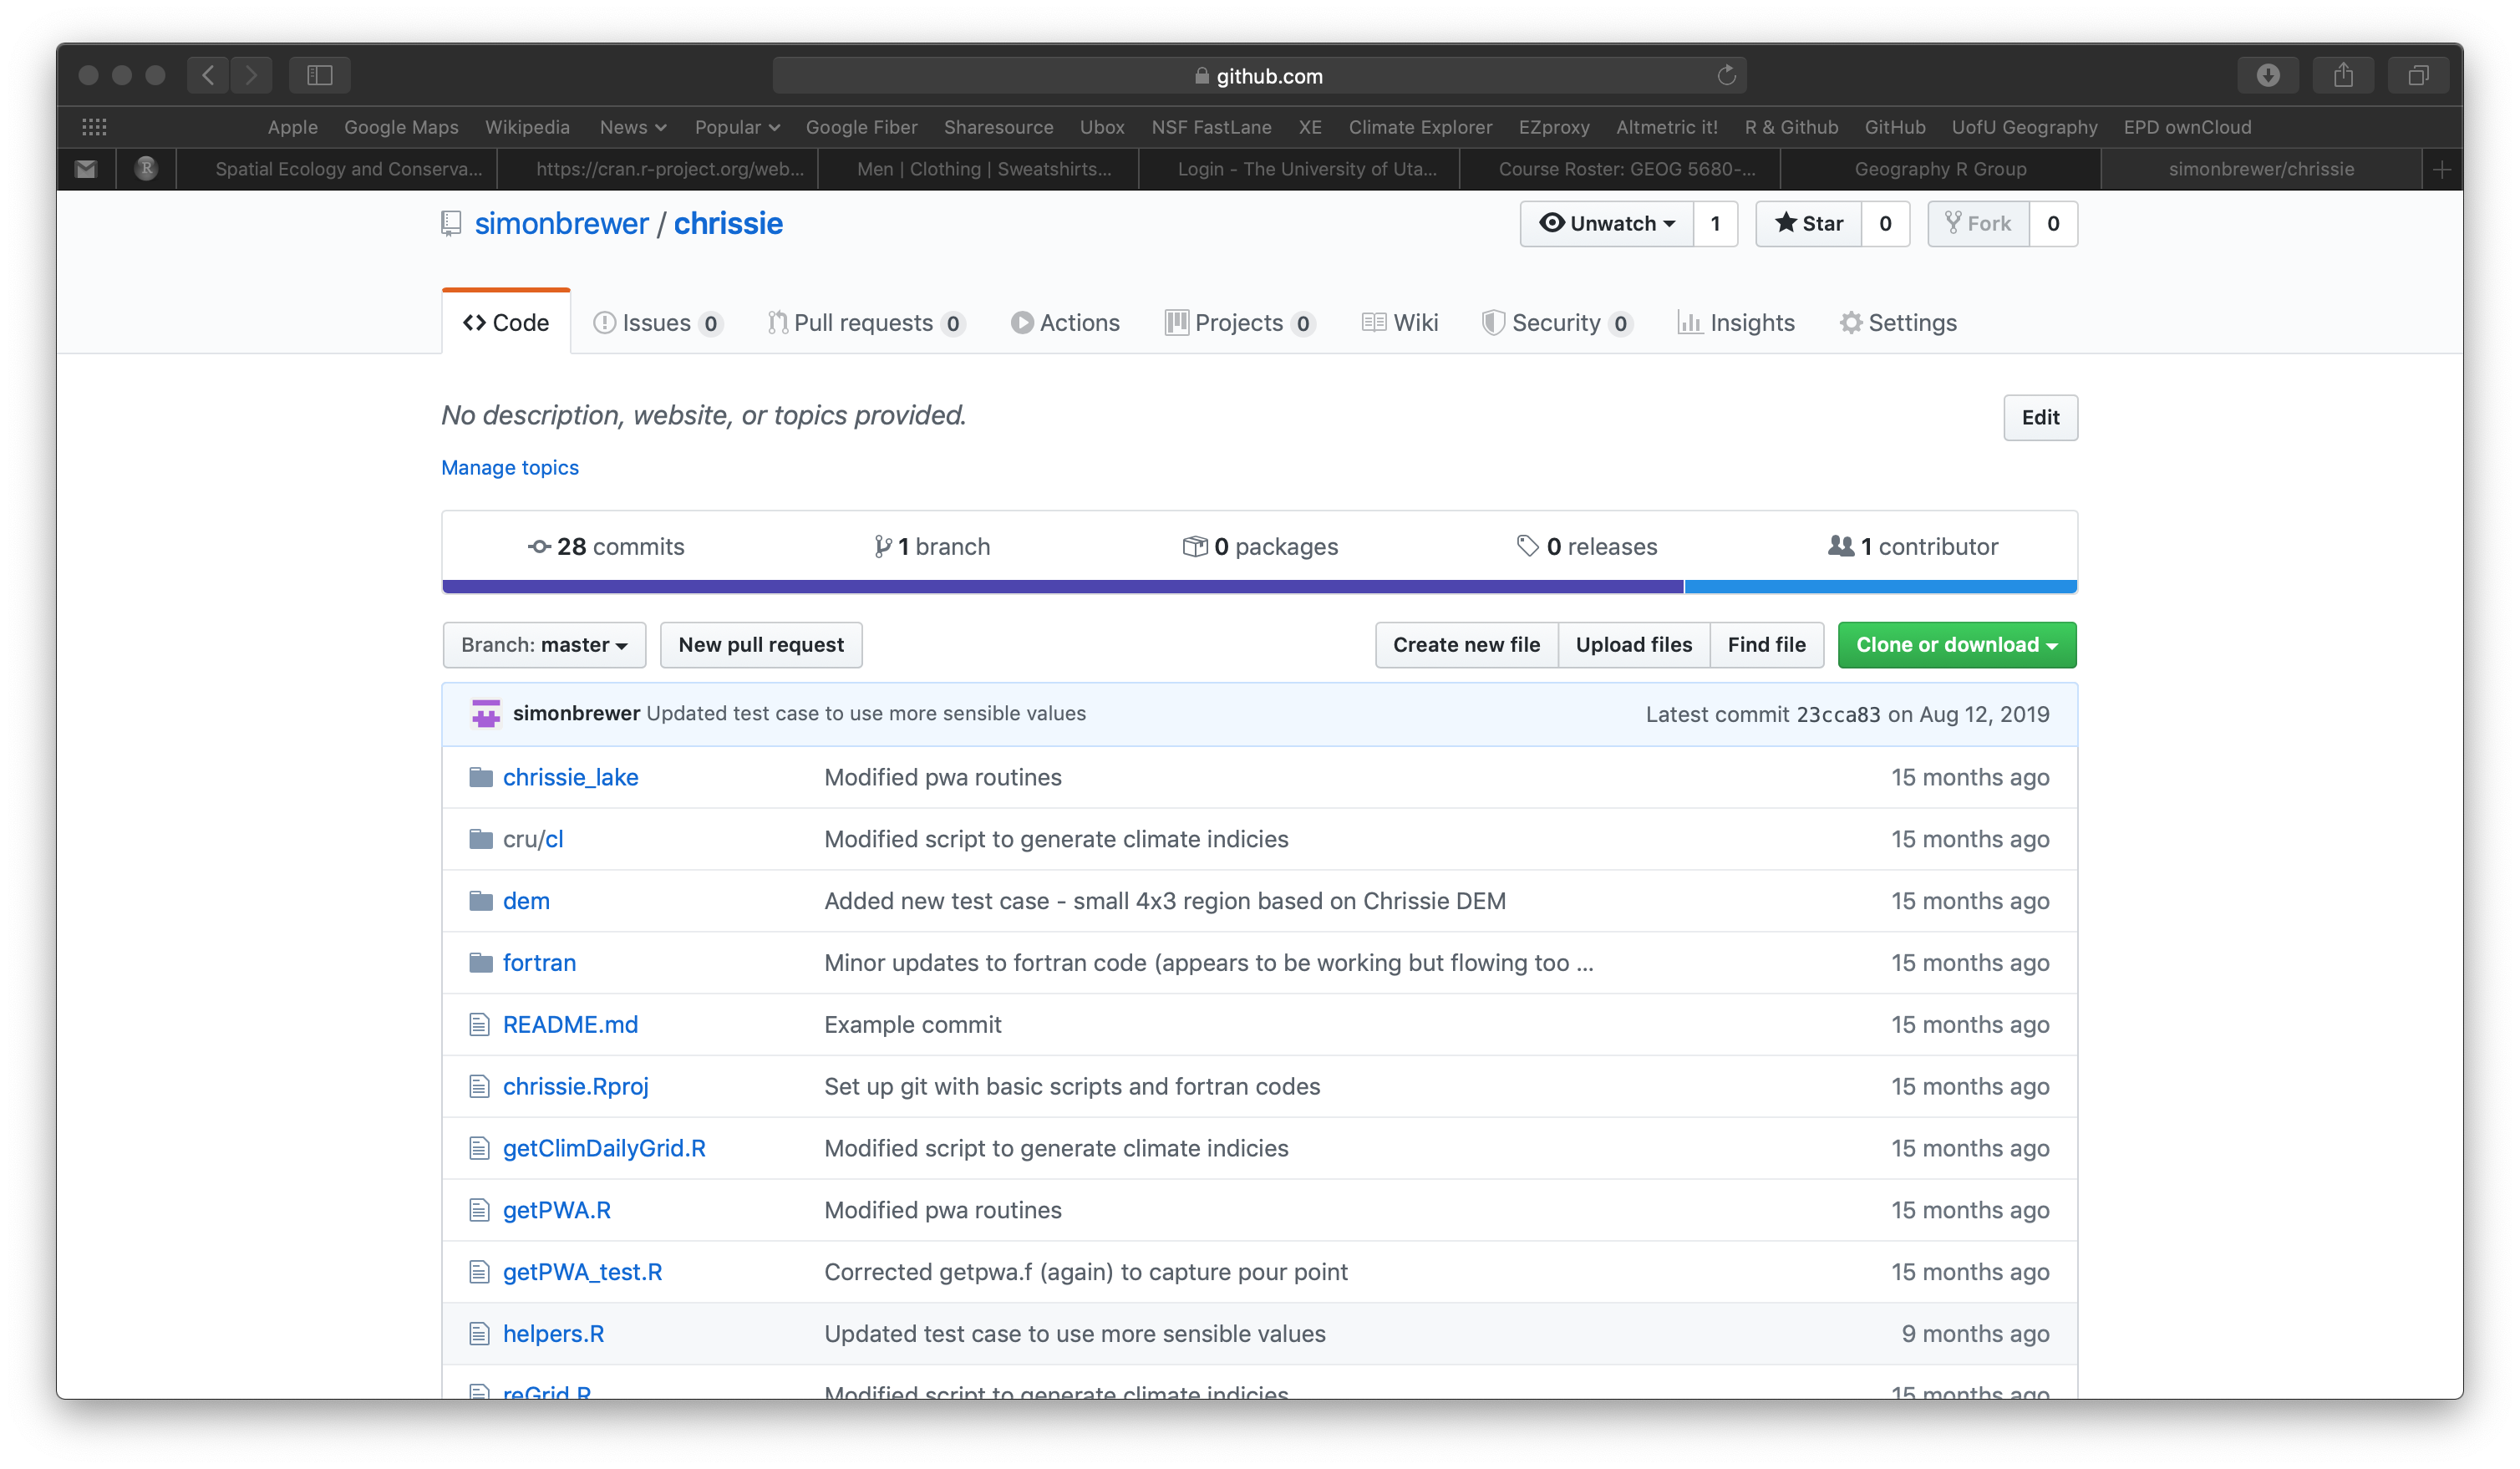
\includegraphics[width=.85\textwidth]{./images/github2.png}
	\end{center}
\end{frame}


\end{document}
